\documentclass{standalone}
\usepackage{tikz}
\usetikzlibrary{patterns, positioning}

\begin{document}
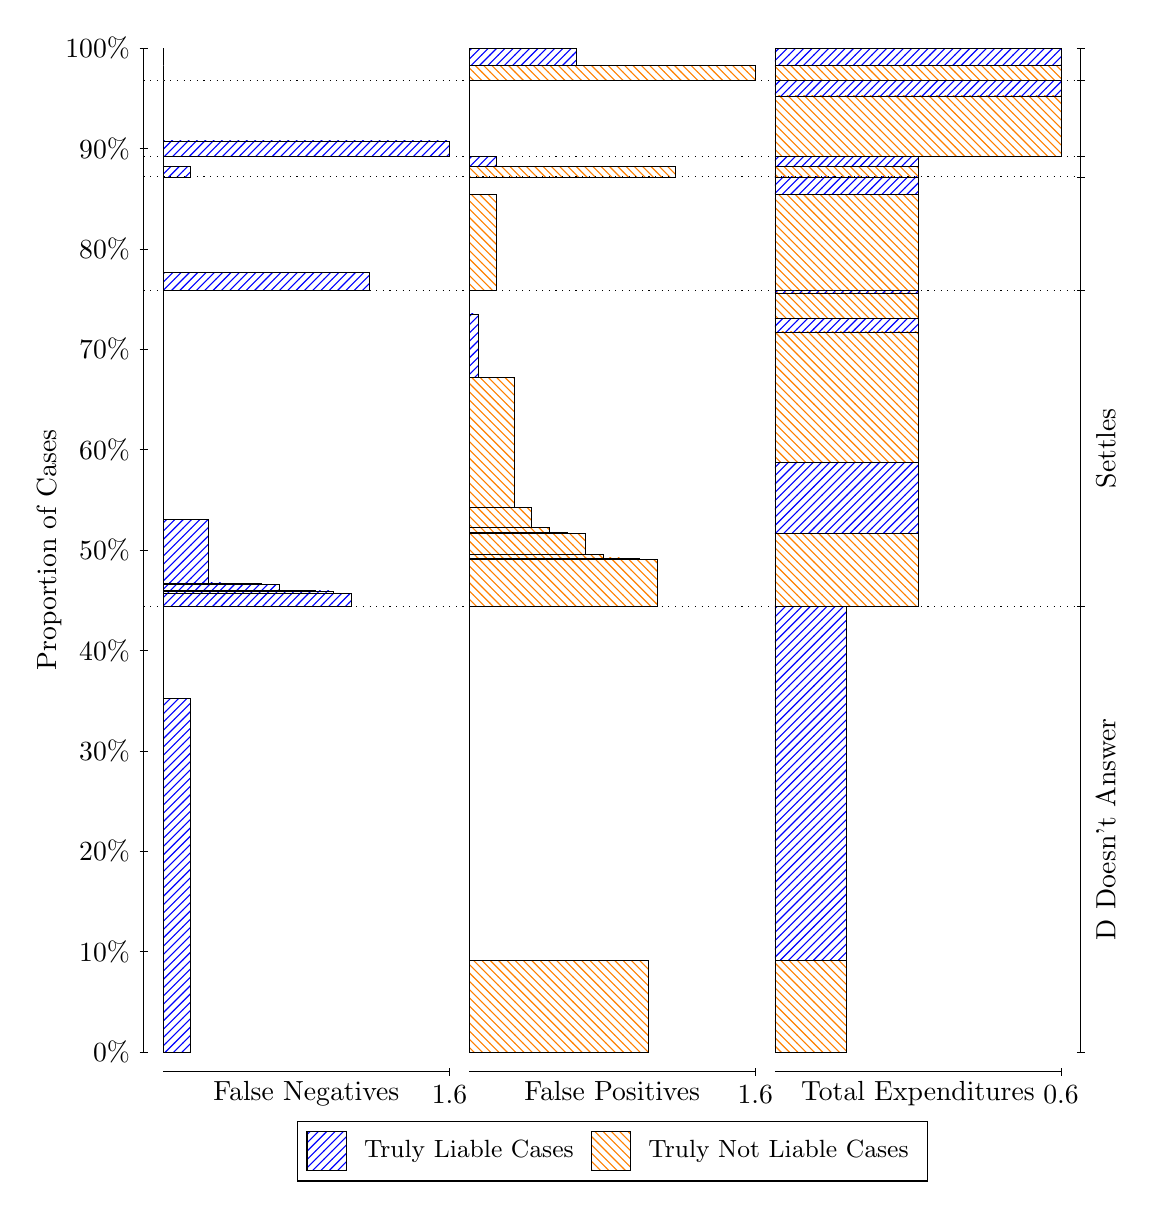
\begin{tikzpicture}
\draw[black, very thin] (1.5,1.75) -- (1.5,14.5);
\node[rotate=90, anchor=center] at (0.3, 8.125) {Proportion of Cases};
\draw[black, very thin] (1.45,1.75) -- (1.55,1.75);
\node[anchor=east] at (1.45, 1.75) {0\%};
\draw[black, very thin] (1.45,3.025) -- (1.55,3.025);
\node[anchor=east] at (1.45, 3.025) {10\%};
\draw[black, very thin] (1.45,4.3) -- (1.55,4.3);
\node[anchor=east] at (1.45, 4.3) {20\%};
\draw[black, very thin] (1.45,5.575) -- (1.55,5.575);
\node[anchor=east] at (1.45, 5.575) {30\%};
\draw[black, very thin] (1.45,6.85) -- (1.55,6.85);
\node[anchor=east] at (1.45, 6.85) {40\%};
\draw[black, very thin] (1.45,8.125) -- (1.55,8.125);
\node[anchor=east] at (1.45, 8.125) {50\%};
\draw[black, very thin] (1.45,9.4) -- (1.55,9.4);
\node[anchor=east] at (1.45, 9.4) {60\%};
\draw[black, very thin] (1.45,10.675) -- (1.55,10.675);
\node[anchor=east] at (1.45, 10.675) {70\%};
\draw[black, very thin] (1.45,11.95) -- (1.55,11.95);
\node[anchor=east] at (1.45, 11.95) {80\%};
\draw[black, very thin] (1.45,13.225) -- (1.55,13.225);
\node[anchor=east] at (1.45, 13.225) {90\%};
\draw[black, very thin] (1.45,14.5) -- (1.55,14.5);
\node[anchor=east] at (1.45, 14.5) {100\%};

\draw[black, very thin] (13.4,1.75) -- (13.4,14.5);
\draw[black, very thin] (13.35,1.75) -- (13.45,1.75);
\node[anchor=west] at (13.35, 1.75) {};
\draw[black, very thin] (13.35,7.408) -- (13.45,7.408);
\node[anchor=west] at (13.35, 7.408) {};
\draw[black, very thin] (13.35,11.425) -- (13.45,11.425);
\node[anchor=west] at (13.35, 11.425) {};
\draw[black, very thin] (13.35,12.863) -- (13.45,12.863);
\node[anchor=west] at (13.35, 12.863) {};
\draw[black, very thin] (13.35,13.126) -- (13.45,13.126);
\node[anchor=west] at (13.35, 13.126) {};
\draw[black, very thin] (13.35,14.085) -- (13.45,14.085);
\node[anchor=west] at (13.35, 14.085) {};
\draw[black, very thin] (13.35,14.5) -- (13.45,14.5);
\node[anchor=west] at (13.35, 14.5) {};

\draw[black, very thin, pattern color=blue, pattern=north east lines] (1.75,1.75) rectangle (2.0906,6.2446);
\draw[black, very thin, pattern color=orange, pattern=north west lines] (1.75,6.2446) rectangle (1.75,7.408);
\draw[black, very thin, pattern color=blue, pattern=north east lines] (1.75,7.408) rectangle (4.1344,7.5783);
\draw[black, very thin, pattern color=blue, pattern=north east lines] (1.75,7.5783) rectangle (3.9073,7.6047);
\draw[black, very thin, pattern color=blue, pattern=north east lines] (1.75,7.6047) rectangle (3.6802,7.6111);
\draw[black, very thin, pattern color=blue, pattern=north east lines] (1.75,7.6111) rectangle (3.4531,7.6136);
\draw[black, very thin, pattern color=blue, pattern=north east lines] (1.75,7.6136) rectangle (3.226,7.687);
\draw[black, very thin, pattern color=blue, pattern=north east lines] (1.75,7.687) rectangle (2.999,7.7003);
\draw[black, very thin, pattern color=blue, pattern=north east lines] (1.75,7.7003) rectangle (2.7719,7.7045);
\draw[black, very thin, pattern color=blue, pattern=north east lines] (1.75,7.7045) rectangle (2.5448,7.7086);
\draw[black, very thin, pattern color=blue, pattern=north east lines] (1.75,7.7086) rectangle (2.3177,8.5138);
\draw[black, very thin, pattern color=orange, pattern=north west lines] (1.75,8.5138) rectangle (1.75,11.425);
\draw[black, very thin, pattern color=blue, pattern=north east lines] (1.75,11.425) rectangle (4.3615,11.651);
\draw[black, very thin, pattern color=orange, pattern=north west lines] (1.75,11.651) rectangle (1.75,12.863);
\draw[black, very thin, pattern color=blue, pattern=north east lines] (1.75,12.863) rectangle (2.0906,12.995);
\draw[black, very thin, pattern color=orange, pattern=north west lines] (1.75,12.995) rectangle (1.75,13.126);
\draw[black, very thin, pattern color=blue, pattern=north east lines] (1.75,13.126) rectangle (5.3833,13.32);
\draw[black, very thin, pattern color=orange, pattern=north west lines] (1.75,13.32) rectangle (1.75,14.085);
\draw[black, very thin, pattern color=orange, pattern=north west lines] (1.75,14.085) rectangle (1.75,14.277);
\draw[black, very thin, pattern color=blue, pattern=north east lines] (1.75,14.277) rectangle (1.75,14.5);
\draw[black, very thin, pattern color=orange, pattern=north west lines] (5.6333,1.75) rectangle (7.9042,2.9133);
\draw[black, very thin, pattern color=blue, pattern=north east lines] (5.6333,2.9133) rectangle (5.6333,7.408);
\draw[black, very thin, pattern color=orange, pattern=north west lines] (5.6333,7.408) rectangle (8.0177,8.0099);
\draw[black, very thin, pattern color=orange, pattern=north west lines] (5.6333,8.0099) rectangle (7.7906,8.0174);
\draw[black, very thin, pattern color=orange, pattern=north west lines] (5.6333,8.0174) rectangle (7.5635,8.0252);
\draw[black, very thin, pattern color=orange, pattern=north west lines] (5.6333,8.0252) rectangle (7.3365,8.0682);
\draw[black, very thin, pattern color=orange, pattern=north west lines] (5.6333,8.0682) rectangle (7.1094,8.3358);
\draw[black, very thin, pattern color=orange, pattern=north west lines] (5.6333,8.3358) rectangle (6.8823,8.3381);
\draw[black, very thin, pattern color=orange, pattern=north west lines] (5.6333,8.3381) rectangle (6.8823,8.3532);
\draw[black, very thin, pattern color=orange, pattern=north west lines] (5.6333,8.3532) rectangle (6.6552,8.4075);
\draw[black, very thin, pattern color=orange, pattern=north west lines] (5.6333,8.4075) rectangle (6.4281,8.6642);
\draw[black, very thin, pattern color=orange, pattern=north west lines] (5.6333,8.6642) rectangle (6.201,10.319);
\draw[black, very thin, pattern color=blue, pattern=north east lines] (5.6333,10.319) rectangle (5.7469,11.125);
\draw[black, very thin, pattern color=blue, pattern=north east lines] (5.6333,11.125) rectangle (5.6333,11.425);
\draw[black, very thin, pattern color=orange, pattern=north west lines] (5.6333,11.425) rectangle (5.974,12.637);
\draw[black, very thin, pattern color=blue, pattern=north east lines] (5.6333,12.637) rectangle (5.6333,12.863);
\draw[black, very thin, pattern color=orange, pattern=north west lines] (5.6333,12.863) rectangle (8.2448,12.994);
\draw[black, very thin, pattern color=blue, pattern=north east lines] (5.6333,12.994) rectangle (5.974,13.126);
\draw[black, very thin, pattern color=orange, pattern=north west lines] (5.6333,13.126) rectangle (5.6333,13.891);
\draw[black, very thin, pattern color=blue, pattern=north east lines] (5.6333,13.891) rectangle (5.6333,14.085);
\draw[black, very thin, pattern color=orange, pattern=north west lines] (5.6333,14.085) rectangle (9.2667,14.277);
\draw[black, very thin, pattern color=blue, pattern=north east lines] (5.6333,14.277) rectangle (6.9958,14.5);
\draw[black, very thin, pattern color=orange, pattern=north west lines] (9.5167,1.75) rectangle (10.425,2.9133);
\draw[black, very thin, pattern color=blue, pattern=north east lines] (9.5167,2.9133) rectangle (10.425,7.408);
\draw[black, very thin, pattern color=orange, pattern=north west lines] (9.5167,7.408) rectangle (11.333,8.3381);
\draw[black, very thin, pattern color=blue, pattern=north east lines] (9.5167,8.3381) rectangle (11.333,9.2386);
\draw[black, very thin, pattern color=orange, pattern=north west lines] (9.5167,9.2386) rectangle (11.333,10.894);
\draw[black, very thin, pattern color=blue, pattern=north east lines] (9.5167,10.894) rectangle (11.333,11.064);
\draw[black, very thin, pattern color=orange, pattern=north west lines] (9.5167,11.064) rectangle (11.333,11.39);
\draw[black, very thin, pattern color=blue, pattern=north east lines] (9.5167,11.39) rectangle (11.333,11.425);
\draw[black, very thin, pattern color=orange, pattern=north west lines] (9.5167,11.425) rectangle (11.333,12.637);
\draw[black, very thin, pattern color=blue, pattern=north east lines] (9.5167,12.637) rectangle (11.333,12.863);
\draw[black, very thin, pattern color=orange, pattern=north west lines] (9.5167,12.863) rectangle (11.333,12.994);
\draw[black, very thin, pattern color=blue, pattern=north east lines] (9.5167,12.994) rectangle (11.333,13.126);
\draw[black, very thin, pattern color=orange, pattern=north west lines] (9.5167,13.126) rectangle (13.15,13.891);
\draw[black, very thin, pattern color=blue, pattern=north east lines] (9.5167,13.891) rectangle (13.15,14.085);
\draw[black, very thin, pattern color=orange, pattern=north west lines] (9.5167,14.085) rectangle (13.15,14.277);
\draw[black, very thin, pattern color=blue, pattern=north east lines] (9.5167,14.277) rectangle (13.15,14.5);
\draw[black, dotted] (1.5,7.408) -- (13.4,7.408);
\draw[black, dotted] (1.5,11.425) -- (13.4,11.425);
\draw[black, dotted] (1.5,12.863) -- (13.4,12.863);
\draw[black, dotted] (1.5,13.126) -- (13.4,13.126);
\draw[black, dotted] (1.5,14.085) -- (13.4,14.085);
\draw[black, very thin] (1.75,1.5) -- (5.3833,1.5);
\node[anchor=north] at (3.5667, 1.5) {False Negatives};
\draw[black, very thin] (5.3833,1.45) -- (5.3833,1.55);
\node[anchor=north] at (5.3833, 1.45) {1.6};

\draw[black, very thin] (5.6333,1.5) -- (9.2667,1.5);
\node[anchor=north] at (7.45, 1.5) {False Positives};
\draw[black, very thin] (9.2667,1.45) -- (9.2667,1.55);
\node[anchor=north] at (9.2667, 1.45) {1.6};

\draw[black, very thin] (9.5167,1.5) -- (13.15,1.5);
\node[anchor=north] at (11.333, 1.5) {Total Expenditures};
\draw[black, very thin] (13.15,1.45) -- (13.15,1.55);
\node[anchor=north] at (13.15, 1.45) {0.6};

\node[black, centered, rotate=90] at (13.72, 4.579) {D Doesn't Answer};
\node[black, centered, rotate=90] at (13.72, 9.4166) {Settles};





\draw (7.449999999999999,1.5) node[draw=none] (baseCoordinate) {};
\begin{scope}[align=center]
        \matrix[scale=0.5, draw=black, below=0.5cm of baseCoordinate, nodes={draw}, column sep=0.1cm]{
            \node[rectangle, draw, minimum width=0.5cm, minimum height=0.5cm, pattern=north east lines, pattern color=blue] {}; &
            \node[draw=none, font=\small] (B) {Truly Liable Cases}; &
            \node[rectangle, draw, minimum width=0.5cm, minimum height=0.5cm, pattern=north west lines, pattern color=orange] {}; &
            \node[draw=none, font=\small] (B) {Truly Not Liable Cases}; \\
            };
\end{scope}

\end{tikzpicture}
\end{document}